\documentclass[tikz,border=5pt]{standalone}
\usepackage{pgfplots}
\pgfplotsset{compat=1.18}
\usepackage{xcolor}

\definecolor{c3blue}{RGB}{100,181,246}
\definecolor{c4magenta}{RGB}{186,85,211}
\definecolor{archgray}{RGB}{220,220,220}

\begin{document}
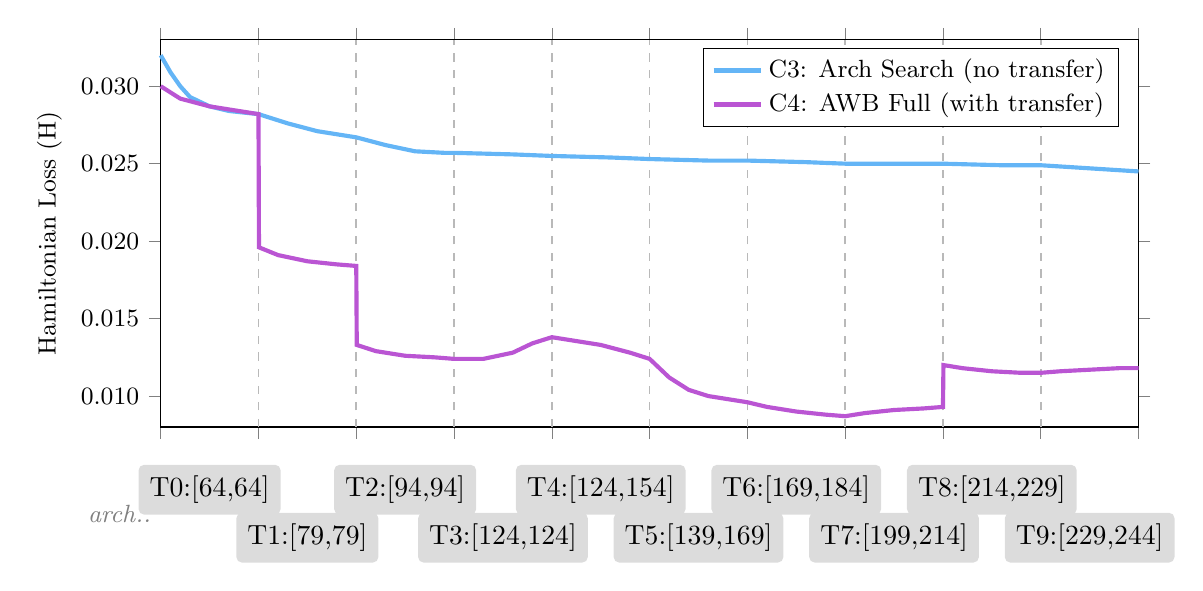
\begin{tikzpicture}

%% ============================================================
%% TOP: combined loss panel — C3 and C4 on same axis
%% ============================================================
\begin{axis}[
  name=loss,
  width=14cm, height=6.5cm,
  axis lines=box,
  clip=false,
  tick align=outside,
  font=\small,
  xmin=0, xmax=100,
  xtick={0,10,20,30,40,50,60,70,80,90,100},
  xticklabels={},
  ylabel={Hamiltonian Loss (H)},
  ymin=0.008, ymax=0.033,
  ytick={0.010,0.015,0.020,0.025,0.030},
  yticklabel style={/pgf/number format/fixed,
                    /pgf/number format/precision=3,
                    /pgf/number format/fixed zerofill},
  scaled y ticks=false,
  legend style={font=\small, at={(0.98,0.98)}, anchor=north east},
]
% task boundary lines
\foreach \bx in {10,20,30,40,50,60,70,80,90}{
  \addplot[dashed, gray!55, forget plot, line width=0.6pt]
    coordinates {(\bx,0.008) (\bx,0.033)};
}
% C3 curve
\addplot[c3blue, line width=1.5pt] coordinates {
  (0,0.0320)(1,0.0309)(2,0.0300)(3,0.0293)(5,0.0287)(7,0.0284)(10,0.0282)
  (13,0.0276)(16,0.0271)(19,0.0268)(20,0.0267)
  (23,0.0262)(26,0.0258)(29,0.0257)(30,0.0257)
  (36,0.0256)(40,0.0255)(46,0.0254)(50,0.0253)
  (56,0.0252)(60,0.0252)(66,0.0251)(70,0.0250)
  (76,0.0250)(80,0.0250)(86,0.0249)(90,0.0249)
  (95,0.0247)(100,0.0245)
};
\addlegendentry{C3: Arch Search (no transfer)}
% C4 curve
\addplot[c4magenta, line width=1.5pt] coordinates {
  (0,0.0300)(2,0.0292)(5,0.0287)(8,0.0284)(10,0.0282)
  (10.05,0.0196)(12,0.0191)(15,0.0187)(18,0.0185)(20,0.0184)
  (20.05,0.0133)(22,0.0129)(25,0.0126)(28,0.0125)(30,0.0124)
  (33,0.0124)(36,0.0128)(38,0.0134)(40,0.0138)
  (42,0.0136)(45,0.0133)(48,0.0128)(50,0.0124)
  (52,0.0112)(54,0.0104)(56,0.0100)(58,0.0098)(60,0.0096)
  (62,0.0093)(65,0.0090)(68,0.0088)(70,0.0087)
  (72,0.0089)(75,0.0091)(78,0.0092)(80,0.0093)
  (80.05,0.0120)(82,0.0118)(85,0.0116)(88,0.0115)(90,0.0115)
  (92,0.0116)(95,0.0117)(98,0.0118)(100,0.0118)
};
\addlegendentry{C4: AWB Full (with transfer)}
\end{axis}

%% ============================================================
%% BOTTOM: shared architecture labels (shown once, large, spaced)
%% ============================================================
\begin{axis}[
  name=archlabels,
  at={(loss.below south west)}, anchor=north west,
  yshift=-0.1cm,
  width=14cm, height=2.8cm,
  xmin=0, xmax=100,
  ymin=0, ymax=1,
  axis lines=none,
  ticks=none,
  clip=false,
  xlabel={Epoch},
  xlabel style={font=\small, yshift=0.3cm},
]
\foreach \bx in {10,20,30,40,50,60,70,80,90}{
  \addplot[dashed, gray!40, forget plot, line width=0.6pt]
    coordinates {(\bx,0) (\bx,1)};
}
% header label on left
\node[font=\small\itshape, gray, anchor=east] at (axis cs:0, 0.5) {arch.:};
% even tasks T0,T2,...,T8  (top sub-row)
\node[fill=archgray, font=\normalsize, inner sep=4pt, rounded corners=2pt]
  at (axis cs:5,  0.75) {T0:[64,64]};
\node[fill=archgray, font=\normalsize, inner sep=4pt, rounded corners=2pt]
  at (axis cs:25, 0.75) {T2:[94,94]};
\node[fill=archgray, font=\normalsize, inner sep=4pt, rounded corners=2pt]
  at (axis cs:45, 0.75) {T4:[124,154]};
\node[fill=archgray, font=\normalsize, inner sep=4pt, rounded corners=2pt]
  at (axis cs:65, 0.75) {T6:[169,184]};
\node[fill=archgray, font=\normalsize, inner sep=4pt, rounded corners=2pt]
  at (axis cs:85, 0.75) {T8:[214,229]};
% odd tasks T1,T3,...,T9  (bottom sub-row)
\node[fill=archgray, font=\normalsize, inner sep=4pt, rounded corners=2pt]
  at (axis cs:15, 0.25) {T1:[79,79]};
\node[fill=archgray, font=\normalsize, inner sep=4pt, rounded corners=2pt]
  at (axis cs:35, 0.25) {T3:[124,124]};
\node[fill=archgray, font=\normalsize, inner sep=4pt, rounded corners=2pt]
  at (axis cs:55, 0.25) {T5:[139,169]};
\node[fill=archgray, font=\normalsize, inner sep=4pt, rounded corners=2pt]
  at (axis cs:75, 0.25) {T7:[199,214]};
\node[fill=archgray, font=\normalsize, inner sep=4pt, rounded corners=2pt]
  at (axis cs:95, 0.25) {T9:[229,244]};
\end{axis}

\end{tikzpicture}
\end{document}
